\section{Methodology}
\dmcmt{
    In same example, we immediately arrive at a better picture. 
    This picture is equivalent to refining and merging back in the Elboher's
setting.}

\dmcmt{ This general part of the paper has this duty: bridge the gap from
whatever gk is doing, that it creates poor quality abstractions with a lot of
singleton neurons, ---> our tree. Answer the question: why and where did the
tree come from. Motivate the tree}

\dmcmt{Two ways of doing this.}

\dmcmt{\textbf{Way 1}: There is a PO (PO1) of all possible merges. GK is
    exploring very small part of it - leads to bad quality, singletons, etc.
    Exploring all of it is hard. But, using semantic info, we can restrict
    ourselves to a smaller part of it, we don't need to explore all of PO1.
    Because, if semantic info tells us that it is better to merge ab than ac,
    then we can discard the entire part of PO1 where ac has been merged. Once
    this cut has been done, we get a tree.
}

\dmcmt{\textbf{Way 2:} GK's ref doesn't produce good quality, and we want a
    better abstraction/refinement by bringing in semantic info. What does
    semantic info give? IO similarity of groups of neurons in \cnc. This gives a
    ordering between possible merge operations, which actually forms a tree.
    Then, each \abs correspond to certain cuts in the tree.
}

\dmcmt{\textbf{Current Decision:} Do way 2, but have 1-2 lines referencing the
    idea in way 1 that says that by following the semantic information we avoid
    exploring all possible \abs
}

\dmcmt{Madhukar supports this. Refiment in our case should be based on priority
    between two merges using semantic info. This priority adds an extra
    dimension. Describe things strictly from the perspective of doing a full
    abstraction then prioritise refinement, don't mix the other perspective of
doing a prioritised abstraction.}

\dmcmt{Get a semantic closeness factor, between pairs of merge groups. Similar
    idea to GK's sameness of color. This gives a natural way to construct a tree
     /PO, and go from there.}

\pagebreak
 
In this work we aim to utilize information from the semantic behavior of \cnc to
better control and guide the refinement process producing higher quality \abs.
In particular, we define a \textit{semantic closeness factor} that captures how
close the semantic-behavior of two groups of neurons are. Then, this closeness
factor can be used to \dmcmt{build a partial order of merge operations?}
prioritise some merges over others. Thus, during the refinement process, we can
cut a merge group \dmcmt{Is it clear what this is?} into subgroups such that
neurons within the same group are semantically closer than neurons across
groups. This allows us to avoid restoring large number of single neurons and
retaining merge groups of higher quality(see Section \ref{s:nn-sam}), achieving
the desired quality of abstraction with a much smaller size. \todo{Ref later
sections}

We show that this closeness factor allows us to arrange the merge operations
into a tree, and the refinement process corresponds to making cuts of this tree.
We then show that the merge groups coming from such cuts have the property that
any two neurons within the group are going to be semantically closer than any
two neurons from two different groups. Thus, we can argue that the refinement
process will partition the neurons in \cnc into groups in a manner that is
optimal with respect to the semantic information.

In the following sections we describe a general framework for such a unified
syntactic and semantic refinement process, describing each component in detail.
\linebreak

Our methodology involves two broad steps:
\begin{enumerate}
    \item Finding a tree structure that represents the order in which neurons should be merged.
    \item Using that structure to guide a CEGAR approach in order to help reduce
        number of refinement steps. \dmcmt{We can't really claim this in any
            way.. but we can claim that we search through a space with higher
        quality \abs, guided by global semantic information.}
\end{enumerate} 

\subsection{Tree and Merges:}


To establish the merging order of neurons, we create a tree 
structure wherein leaf nodes represent the original neurons, and 
non-leaf nodes represent merge groups. The construction of the tree 
follows a bottom-up approach, prioritizing the merging of similar neurons 
and delaying the merging of dissimilar ones. Similarity is ascertained through 
observation vectors.

\begin{figure}[H]
    \centering
    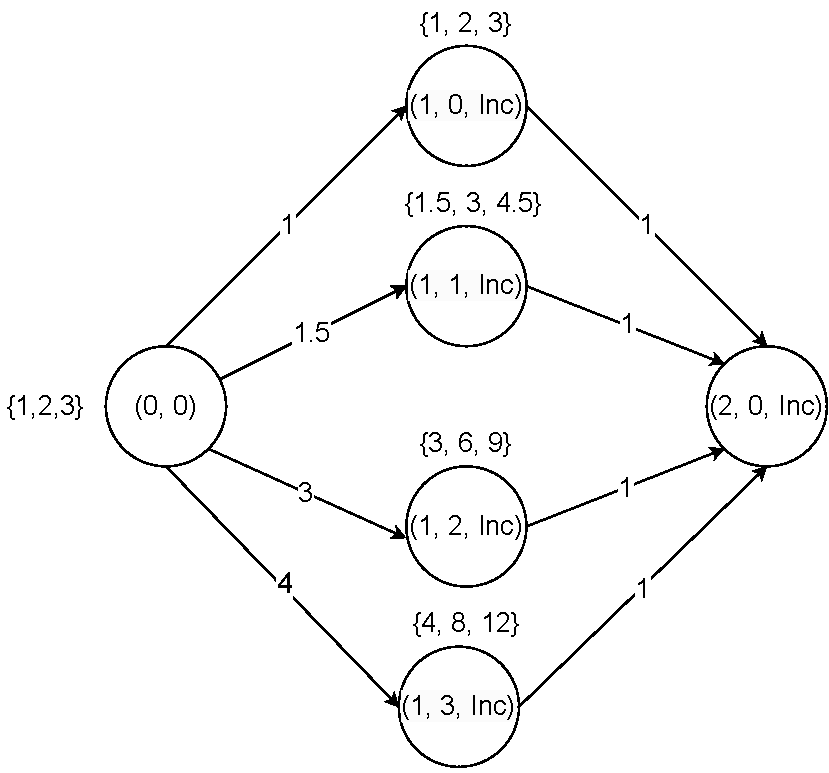
\includegraphics[width=0.5\textwidth]{diagrams/tree_merges.pdf}
    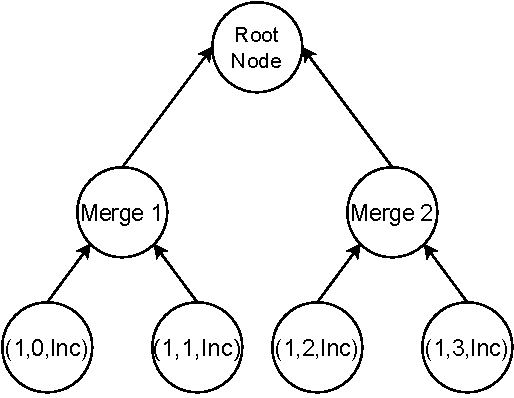
\includegraphics[ width=0.47\textwidth]{diagrams/Order_of_Merge.pdf}
    \caption{Order Of Merging}
    \label{Figure: Order Of Merging}
\end{figure}

In figure \ref{Figure: Order Of Merging}, if we give the list of input vectors $[[1], [2], [3]]$ to the observation function $o_{(i, j)}$ for $(n_{(1, 1, Inc)})$, then we obtain a list of output vectors $[[1.5], [3], [4.5]]$. We utilize the output of the observation function as a measure to merge neurons. For instance, considering three neurons $n_{(w, i)}$, $n_{(w, j)}$, and $n_{(w, k)}$ with 
observation vectors $o_{(w, i)}$, $o_{(w, j)}$, and 
$o_{(w, k)}$, the merging sequence adheres to the following conditions: 

If $||o_{(w, i)} - o_{(w, j)}||_{2} \leq ||o_{(w, i)} - 
o_{(w, k)}||_{2}$ and $||o_{(w, i)} - o_{(w, j)}||_2 \leq ||o_{(w, j)} - 
o_{(w, k)}||_{2}$, then $n_{(w, i)}$ and $n_{(w, j)}$ are initially merged into a 
representative neuron $\alpha$, followed by the merging of $\alpha$ and $n_{(w, k)}$. 
Here $||o_{(w, i)} - o_{(w, j)}||_{2}$ computes the ``$\textit{Euclidean 
Distance}$" between the observation vectors $o_{(w, i)}$ and  $o_{(w, j)}$.


In Figure \ref{Figure: Order Of Merging}, for the first layer, the initial 
merge would involve the neuron $n_{(1, 0, Inc)}$ with $n_{(1, 1, Inc)}$, 
forming $\textit{Merge 1}$, then we would combine $n_{(1, 2, Inc)}$ and 
$n_{(1, 3, Inc)}$, forming $\textit{Merge 2}$. Finally we combine 
$\textit{Merge 1}$ and $\textit{Merge 2}$ into the root node. 

As we progress up the tree, the degree of over-approximation rises. 
This is due to the increasing difference between observation vectors as 
we ascend. Therefore, the sub-trees closer to the root are indicative of 
coarser merges, whereas the ones farther from the root represent finer merges. 

\sncmt{Do we need to say how this tree corresponds to all possible merge groups which are allowed in the partial order because different cuts in the tree correspond to different neural networks. If ``Yes'', do we need to include the Guy Katz abstraction details. And then, in the next section, do we need to tell how to construct the actual weight matrix from indexing into this all possible merge groups weight matrix? Because Dig talked about efficient data structures in the intro.}

\subsection{Using examples to make cuts in the Tree} 
We are guided by this tree as a prospective refinement method. Starting with the 
entire tree where everything is merged. We leverage it to refine the network.
This process commences by identifying the ``culprit neuron $\gamma$'' 
selected for refinement. A ``culprit neuron'' in a merge group is selected 
on the basis of how much the neuron contributed to the output. If change in 
output of  neuron changes the value of the output neuron significantly then
that neuron is a good candidate for ``culprit neuron". 

Following this, we reverse all merges dependent on the culprit 
neuron $\gamma$. Therefore, refinement essentially involves finding a 
cut-point in the tree, precisely where all merges dependent on the 
culprit neuron $\gamma$ are undone. Each cut produces a set of trees, 
the merge groups then consist of neurons in the leaf nodes of the  these trees.
Therefore finding new merge groups for refinement is therefore just finding a 
cuts in the tree.

\sncmt{Do we need to tell the LCA algorithm here?}

\begin{figure}
    \centering
    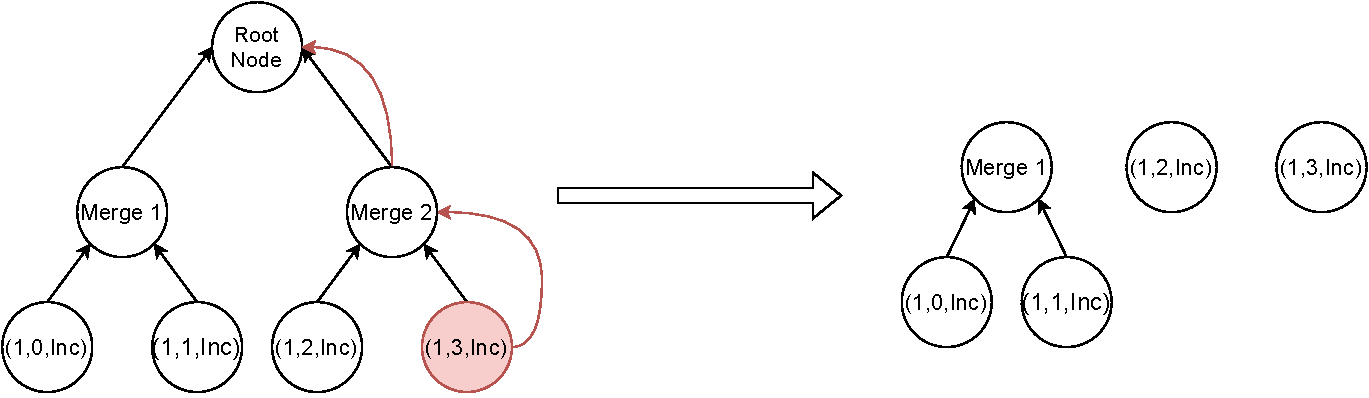
\includegraphics[width = 0.5\textwidth]{diagrams/before_and_after_cut_2.pdf}
    \caption{Trees and Cuts}
    \label{Figure 2}
\end{figure}

Consider Figure \ref{Figure 2}, illustrating the merging sequence of neurons $n_{(1,0,Inc)}$, $n_{(1,1,Inc)}$, $n_{(1,2,Inc)}$, and $n_{(1, 3, Inc)}$. If, for instance, the neuron $n_{(1,3,Inc)}$ is identified as the problematic neuron based on a counter-example, we will reverse all the merges dependent on the $n_{(1,3,Inc)}$ neuron, including $\textit{Merge 2}$ and the $\textit{Root Node}$ merge. Consequently, after implementing this reversal indicated in Figure \ref{Figure 2}, our refinement phase will yield three distinct merge groups. The first merge group comprises two neurons, namely $n_{(1,0,Inc)}$ and $n_{(1,1, Inc)}$. The second merge group and the third merge have single neurons $n_{(1,2, Inc)}$ and $n_{(1,3,Inc)}$, respectively.

\subsection{Culprit Neurons} 

A neuron, denoted as $\gamma$, is designated as a culprit neuron within a
specific layer when absolute value of the product of the difference between
$(v_{Rep(\gamma)}$ and $v_{\gamma})$ and the effective weight is maximized.
\todo{Add the 3 different methods generating counter-examples. Scores should be
avg over $\beta$ for a particular $\gamma$.}

$||(v_{Rep(\gamma)} - v_{\gamma})||_{2} \cdot |(\textit{effective\_weight})|$

In this context, $Rep$ signifies the representative neuron for neuron $\gamma$, $v_{\gamma}$ represents the value of the neuron $\gamma$ at counter-example $\beta$ and $\textit{effective\_weight}$ represents the how much does the value of output neuron changes with respect to change in the value of the neuron under consideration, essentially corresponding to the ``$\textit{gradient}$'' at that particular example ``$\beta$''.

\begin{algorithm}
    \caption{Finding Cuts in the Tree (find\_new\_merge\_groups)}
    \begin{algorithmic}[1]
        \State $\gamma= \arg \max_i \|v_{Rep(i)} -v_i \|_2 \cdot | \textit{effective\_weight}| $ 
        \State Find a sequence of nodes, $t_1,t_2,t_3,..,t_k$ representing a  path from $t_1=$root to $t_k=\gamma$.
        \State Remove the nodes $t_1,t_2,..,t_{k-1}$ denoting the merges dependent on $\gamma$ through this path, leading to our connected tree being split into a collection of disconnected sub-trees.
        \State New merge groups are the leaf nodes in our disconnected graph.
    \end{algorithmic}
    \hspace*{\algorithmicindent} \textbf{Output} New Merge Groups
\end{algorithm}

\subsection{Optimality of the Trees}
Our objective is to determine the most efficient order for merging neurons, minimizing the introduction of over-approximation at each step. This approach aims to avoid creating networks with excessive over-approximation, which could lead to the generation of spurious counter-examples in response to queries. Opting not to mitigate over-approximation at each step would result in an increased number of refinement steps. This essentially entails making additional solver calls, incurring significant costs to eliminate the spurious counter-examples.


Nevertheless, during the initial merging process (until saturation is reached), the root node ``$\rho$'' will exhibit the same level of over-approximation across all conceivable merging scenarios—for all possible tree sequences. Nevertheless, when we descend one level down the tree to explore the children nodes of our original root node $\rho$ for the purpose of identifying a cut for refinement, we discover varying levels of over-approximation manifesting in the root nodes of the resultant sub-trees. These differences are a result of the different merging scenarios pursued to construct those individual trees.

\begin{algorithm}[H]
\caption{Cluster Merging Algorithm (find\_abstraction\_tree)}
\label{Cluster Merging Algorithm}
\begin{algorithmic}[1]
    \State Initialize every simulated distance vector as a singleton cluster.
    \State Initialize $C=\{v_1,v_2,v_3,..\}$ as the set of singleton clusters.
    \State Initialize a Binary Tree $T$ with leaves as $\{(n_1),(n_2),(n_3),..\}$ corresponding to $\{v_1,v_2,v_3,..\}$.
    \State Initialize $V$ as a set of visited nodes, empty at first.
    
    \Function{MergeFunction}{$u, v$}
        \If{All nodes are classified as \textbf{Inc}}
        {
        
            \Return $\max(u, v)$
        }
        \Else{ }
        {
        
            \Return $\min(u, v)$
        }
        \EndIf
    \EndFunction
    
    \While{$|C|>1$}
        \State $v_j, v_j = \arg\min_{\substack{a, b \in C}} \| a - b \|_2$
        \State Set $w=\text{MergeFunction}(v_i,v_j)$
        \State Let nodes from $T$ not in $V$ corresponding to $v_i,v_j$ be $m_i$ and $m_j$
        \State Remove $v_i,v_j$ from $C$ and add $w$ to $C$.
        \State Make $(m_i \cup m_j)$ the parent of $(m_i)$ and $(m_j)$ in tree $T$
        \State Add $m_i$ and $m_j$ to $V$.
    \EndWhile
\end{algorithmic}
\end{algorithm}

While the optimal tree, representing the optimal merging sequence, can aid in the refinement process by guiding the reversal of merges, finding such an optimal tree poses is extremely challenging. Even when dealing with only `n' Increment (Inc) neurons that have been merged to saturation, the total number of possible trees is given by $(2n-3)!!$, making the task of determining the truly optimal tree from these options extremely challenging.

Since finding this ideal tree is a challenging task, we employ hierarchical clustering (Algorithm \ref{Cluster Merging Algorithm}) as an approach to approximate and derive such a tree. Initially, we simulate our network using a set of `$k$' inputs. Subsequently, we employ cluster analysis on these `$k$' points to construct a hierarchical arrangement of clusters. This process initiates with data points corresponding to simulated values (observation values in the observation vector) of a neuron  forming their own cluster. The clusters are then systematically combined based on their similarity, thereby generating a hierarchy of clusters. The choice of similarity measure is the ``$distance \hspace{1mm} metric$" between clusters. We have used ``$Euclidean \hspace{1mm} Distance$" as our distance metric. Given that the data points to perform this hierarchical clustering originate from the values of the simulated neurons, this hierarchical clustering effectively reflects the methodology we employ to merge the neurons.

For example, in Figure \ref{Figure: Order Of Merging}, we conducted a simulation of our network on three data points. Subsequently, we examined the observation vectors corresponding to these points. Utilizing the hierarchical clustering algorithm, the initial selection for merging  will involve $(n_0^{1}, Inc)$ and $(n_1^{1}, Inc)$ because of the fact that their Euclidean distance is minimum. This forms $\textit{Merge 1}$ in Figure \ref{Figure: Order Of Merging}. The observation vector for $\textit{Merge 1}$ ($\nu_\textit{Merge1 }$) is the max of the $\nu((n_0^{1}, Inc))$ and $\nu((n_1^{1},Inc))$ which is \{1.5, 3, 4.5\}. For decrement nodes the observation vector would be minimum of the observation vector of the corresponding decrement nodes. The next merging step involved selecting $\nu((n_2^{1}, Inc))$ and $\nu((n_3^{1}, Inc))$ and merging these two neurons, representing $\textit{Merge 2}$ in Figure \ref{Figure: Order Of Merging}. The observation vector for $\textit{Merge 2}$ is now \{4, 8, 12\}. Ultimately, the Merge1 merge group is merged with the $\textit{Merge 2}$ merge group to create the Root Node in our network.

\begin{figure}[H]
    \centering
    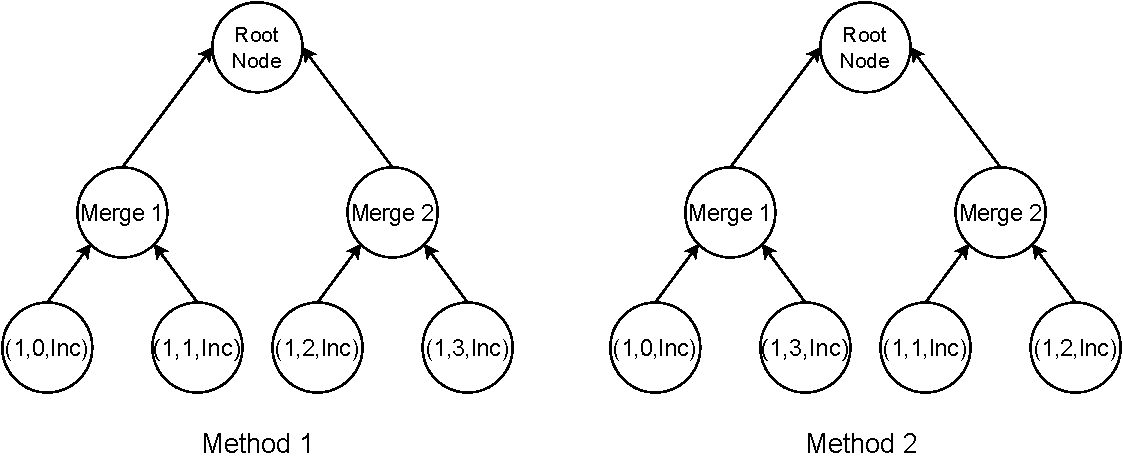
\includegraphics[width = 0.5\textwidth]{diagrams/good_vs_bad_merges.pdf}
    \caption{Ways of Merging}
    \label{Figure 3}
\end{figure}

This approach of merging neurons based on similarity proves advantageous as it helps in reducing number of refinement steps. For instance, consider the task of checking whether $\forall v_{0}^{0} \in [0, 1]$ implies $v_{0}^{2} < 10$. If we had the neuron $(n_{3}^{1}, Inc)$ as the culprit neuron and then if we follow the second merging approach depicted in Figure \ref{Figure 3}, then we would have been compelled to reverse both $\textit{Merge 1}$ and $\textit{Merge 2}$. However, by employing the first merging approach, undoing only the $\textit{Merge 2}$ becomes sufficient, resulting in a reduction in the number of refinement steps required.


\subsection{Overall Algorithm}
\begin{algorithm}[H]
    \caption{Overall Algorithm}
    \label{Overall Algorithm}
    \begin{algorithmic}[1]
        \State $\mathcal{N'}$ = split\_Inc\_Dec($\mathcal{N}$)
        \State $\mathcal{N''}$ = abstract\_network($\mathcal{N'}$)
        \State simulation\_dict = simulate\_network($\mathcal{N'}$)
        \State $\mathcal{T}$ = find\_abstraction\_tree($\mathcal{N'}$, $simulation\_dict$)
        \If{verify($\mathcal{N''}$, $\kappa$, $\lambda$) is UNSAT}{

            \Return Property Holds
            }
        \Else
            \State Extract counter-example $\beta$
            \If{$\beta$ is not a spurious counter-example}
            {

                \Return ($\beta$, Property Violated)
            }
            \Else
                \State Find culprit neuron $\gamma$
                \State $merge\_groups$ = find\_new\_merge\_groups($\mathcal{T, \gamma}$)
                \State $\mathcal{N''} = get\_abstract\_network(merge\_groups)$
                \State \textbf{goto} step 5
            \EndIf
        \EndIf
    \end{algorithmic}
\end{algorithm}
